
% Experimental:
\renewcommand{\subsubsection} {\textsl{ }\\ }

\chapter{Overview}
\index{overview}
This chapter provides a brief overview of the Tinn-R project.

\newpage
\hypertarget{overview_quickstart}{}
\section{Quick start}
\index{overview!quick start}

Let's say you don't have time to read the full user guide just yet.
That's OK, we know it is huge, so let's just give you a few tips on how to get started:

\begin{itemize}
  \item If your version is the same or above 3.0.1.0, Tinn-R does not require any special configuration.
      That is, the program is ready to be used. One important thing to be done before using it:
      set a \RR{} mirror as close as possible to where you work. For that, first click on \texttt{CTRL + F8}.
      This opens the \texttt{Tools} window, then click on \texttt{R/Mirrors}.
      Select the \RR{} mirror and push the button that shows an hourglass in the taskbar.
      The chosen repository will be the new default for all actions dependent repository
      (install packages, upgrade packages, etc);
  \item If your version is the below the 3.0.1.0, read the \htmladdnormallink{basic instructions to install and
      configure}{\#basic\_configuration\_installconfigure} \RR{} and Tinn-R:
    \texttt{it's a small and easy to follow document};
  \item Choose either Rgui or Rterm: \texttt{it takes one mouse click};
  \item Open \textit{Help/Example of script.R}: \texttt{another
      mouse click};
  \item Use the \textit{R toolbar} to control \RR{}: \texttt{it only takes one
      mouse click for each action};
  \item Have fun!
\end{itemize}

If you have any questions we suggest you consult this user guide.


\section{What is Tinn-R?}
\index{overview!what is Tinn-R?}

\begin{figure}[H]
  \begin{center}
    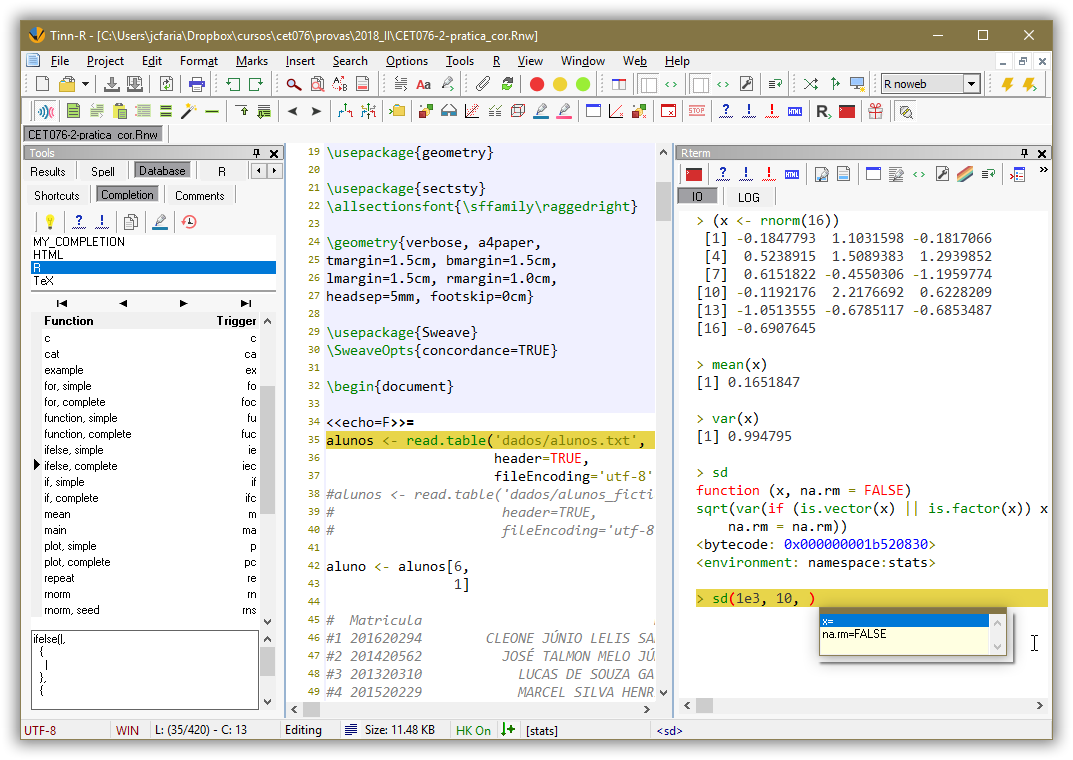
\includegraphics[width=\headwidth]{./res/general.png}
  \end{center}
  \caption{Tinn-R screenshot.}
  \label{fig:tinn-r_screenshot}
\end{figure}

\htmladdnormallink{Tinn}{http://tinn.solarvoid.com} is a small ASCII file 
editor primarily intended as a better replacement for the default Notepad 
running under the Windows OS. The name is the recursive acronym: 
\underline{T}inn \underline{i}s \underline{n}ot \underline{N}otepad.

\htmladdnormallink{Tinn-R}{https://nbcgib.uesc.br/tinnr/en/}
(Figure \ref{fig:tinn-r_screenshot})
is an extension of the original Tinn editor (ASCII and UNICODE), providing additional functionality
to control \htmladdnormallink{R}{http://cran.r-project.org} running as Rgui 
(in SDI mode), Rterm and 
\htmladdnormallink{JGR}{http://stats.math.uni-augsburg.de/JGR/} 
and a whole lot of additional resources.

Tinn-R can also be thought of as feature-rich replacement of the basic 
script editor provided with Rgui. It provides syntax-highlighting, code 
submission as a whole or line-by-line, in addition to many other useful 
tools to ease the writing and debugging of \RR{} code.

Both Tinn and Tinn-R are distributed under the 
\htmladdnormallink{GPL 2}{http://www.gnu.org/copyleft/gpl.html} license or above.


\hypertarget{overview_whytinnr}{}
\section{Why Tinn-R?}
\index{overview!why Tinn-R?}

Do you:

\begin{itemize}
  \item like the open source initiative?
  \item need a simple but powerful GUI/Editor for the \RR{} environment?
  \item enjoy the ability to have syntax highlighting in your source code?
  \item need a tool that is simple to use but with the capabilities of a mighty editor?
  \item need a tool to work with plain text files?
  \item need a tool with simple commands for working with LaTeX, Sweave and Txt2tags?
  %\item want to have access to the functionality of commercial and professional products but without having to pay for it?
  \item want to have access to the functionality of commercial and professional products?
\end{itemize}

\textit{\textbf{If you have answered YES to any of the questions above, then Tinn-R is a good option for you!}}


\hypertarget{overview_whatdoyouget}{}
\section{What do you get by using Tinn-R?}
\index{overview!what do you get?}

\begin{itemize}
  \item The ability to communicate with the \RR{} environment by sending
    instructions, controling its processing, and receiving results:
    \begin{itemize}
      \item Rterm.exe
      \item Rgui.exe
      \item JGR
    \end{itemize}
  \item Projects:
    \begin{itemize}
      \item Create project files to organize your work including 
        one level of sub-folders and automatic file name sorting
      \item Easy project management in graphical and text modes
    \end{itemize}
  \item Work with unlimited length files
  \item Work on multiple documents at the same time, choosing 
    between multiple-document interface (MDI) and tabbed 
    document interface (TDI)
  \item Single-document window splitting
  \item Support to macros (volatile):
    \begin{itemize}
      \item Record
      \item Playback commonly used sequences
    \end{itemize}
  \item Search and replace not restricted to your active file, but 
    also extendable to all open files, all project files, or any 
    folder
  \item View file differences with color highlighting
  \item Syntax highlighting, which can be set by file type
  \item Spell checking
  \item Multiple undo/redo
  \item Highlighted color syntax with print preview
  \item Ability to select:
    \begin{itemize}
      \item Normal
      \item Column
      \item Lines
    \end{itemize}
  \item Ability to bookmark:
    \begin{itemize}
      \item Line
      \item Block
    \end{itemize}
  \item Line numbers
  \item Special characters
  \item Sort multiple variable types:
    \begin{itemize}
      \item String
      \item Data
      \item Number
    \end{itemize}
  \item Count:
    \begin{itemize}
      \item Character
      \item Words
      \item Spaces
    \end{itemize}
  \item ASCII chart
  \item Export with highlight to clipboard:
    \begin{itemize}
      \item RTF
      \item HTML
      \item TeX
    \end{itemize}
  \item Matching bracket highlighting
  \item Conversion tools:
    \begin{itemize}
      \item Pandoc
      \item Deplate
      \item Txt2tags
    \end{itemize}
  \item LaTeX support:
    \begin{itemize}
      \item Edition
      \item Compilation
      \item Inverse DVI search.
    \end{itemize}
\end{itemize}

We are constantly on the move!


\section{Do I have to pay for Tinn-R?}

%Absolutely NOT! It's free as in beer and licensed under GPL.
%
%
%However, since creating and maintaining the project involve many costs, donations are welcome!
%
%If you wish to express your appreciation and to make
%a donation, click on the \texttt{Help/About/Version/Donate} icon or follow
%this link: \htmladdnormallink{Donation}{https://www.paypal.com/cgi-bin/webscr?cmd=_s-xclick&hosted_button_id=B5GDCSVXH6JV4}.

The Tinn-R Team have been developing Tinn-R project under the GPL since june of 2003 (almost 15 years).
All this time it was distributed as free software. Currently, there are corporative
alternatives (paid or free as RStudio and RTVS) to lead with R environment. So, to cover the costs,
we are evaluating the possibility that it will be distributed as sharewere in the near future.


\section{What was the motivation to start and maintain the Tinn-R project?}

\begin{description}
  \item[Motivation to start Tinn-R:]
    We could not find a GUI/Editor for \RR{} running in the Windows OS that
    would give us all the ease of use and flexibility we wanted. So, we 
    started this project using an open source editor called 
    \htmladdnormallink{Tinn}{http://tinn.solarvoid.com} as our initial 
    platform.
  \item[Motivation to maintain Tinn-R:]
    The most difficult phase of the project was getting started: choosing
    the editor; all the preliminary performance and stability tests;
    understanding source structure; among many other struggles. Making
    it to run more and more smoothly and according to our daily needs was
    then a natural consequence. This is all to say that the open source
    movement has substantially changed our lives for better. We strongly
    believe in making software more widely available so that more people
    can benefit from it. We consider Tinn-R to be our small contribution
    to this fantastic open source initiative.
\end{description}


\section{What is the sentence that we, from the development team, most like to hear?}

Tinn-R made my life easier ... thanks for creating it.

% I wonder the below it is not necessary to the ebook! jcfaria
%\section{Which tools were used to create this user guide?}

%\begin{itemize}
%  \item Tinn-R was used to:
%    \begin{itemize}
%      \item Organize all source files under our project directory;
%      \item Edit the Txt2tags source files;
%      \item Manage the conversion and visualization of the final HTML code;
%    \end{itemize}
%  \item To manage external resources available within Tinn-R we used the following:
%    \begin{itemize}
%      \item Txt2tags, a python script to make the conversion from Txt2tags to HTML;
%      \item Python interpreter;
%      \item CSS to create the layout of the HTML content;
%    \end{itemize}
%  \item Pictures:
%    \begin{itemize}
%      \item \htmladdnormallink{IrfanView}{http://www.irfanview.com/} was used
%        to select areas of the figures created using print screen function.
%    \end{itemize}
%\end{itemize}

%\begin{quotation}
%  That was all!
%\end{quotation}

%This user guide can be easily converted to the following formats: HTML, 
%XHTML, SGML, LaTeX, Lout, UNIX man page, Wikipedia, Google Code Wiki, 
%DokuWiki, MoinMoin, MagicPoint (mgp), and PageMaker. Just use the 
%Tinn-R GUI/Editor to do that.


\section{Acknowledgment}

We would like to thank those who have assisted us with the Tinn-R project, 
either by sending suggestions or by contributing to its development.


\section{Feedback, suggestions and bug reports}
\index{overview!bug reports}

Please submit feedback to 
\htmladdnormallink{Jos� Cl�udio Faria}{mailto:joseclaudio.faria@gmail.com}. 
If you submit a bug report, please provide as much detail as possible. This 
includes indicating the Tinn-R version, your operating system (Windows XP, 
Windows 7, etc) and language (English, French, Portuguese). If the bug is 
related to an interface with \RR{}, please also indicate which version of \RR{}
you are using, as well as whether you are running Rterm or Rgui. Ideally, 
please also add the content of the \textit{Tools/Results/Ini log} interface 
since this will help us address the issue more promptly.

\section{What tools were used to make this guide?}

It were used mainly:
\begin{enumerate}
   \item \htmladdnormallink{Tinn-R}{https://nbcgib.uesc.br/tinnr/en/}
    to edit, manager (as project) and submit to compilation the \LaTeX~source files;
   \item \htmladdnormallink{\TeX studio}{http://texstudio.sourceforge.net/}
    was also used in some parts where, to improve the productivity, it was necessary a more specialized \LaTeX~editor;
   \item \htmladdnormallink{Vim}{http://www.vim.org/}
    and 
    \htmladdnormallink{\LaTeX Box plugin}{https://github.com/LaTeX-Box-Team/LaTeX-Box}
    when working under openSUSE (the actual preferred OS of the Tinn-R project coordinator);
   \item \htmladdnormallink{WinSnap}{http://www.ntwind.com/software/winsnap.html}
    to get all images from the application;
   \item \htmladdnormallink{FastStone Image Viewer}{http://www.faststone.org/}
    to browser and manager images;
   \item \htmladdnormallink{R}{http://www.r-project.org/}
    as interpreter;
   \item \htmladdnormallink{Mik\TeX}{http://miktex.org/}
    to compile the \LaTeX~source files to final PDF format;
   \item \htmladdnormallink{SumatraPDF}{http://blog.kowalczyk.info/software/sumatrapdf/free-pdf-reader.html} as PDF viewers.
\end{enumerate}
